% $Header: /Users/joseph/Documents/LaTeX/beamer/solutions/conference-talks/conference-ornate-20min.en.tex,v 90e850259b8b 2007/01/28 20:48:30 tantau $

\documentclass[10pt]{beamer}

% This file is a solution template for:

% - Talk at a conference/colloquium.
% - Talk length is about 20min.
% - Style is ornate.



% Copyright 2004 by Till Tantau <tantau@users.sourceforge.net>.
%
% In principle, this file can be redistributed and/or modified under
% the terms of the GNU Public License, version 2.
%
% However, this file is supposed to be a template to be modified
% for your own needs. For this reason, if you use this file as a
% template and not specifically distribute it as part of a another
% package/program, I grant the extra permission to freely copy and
% modify this file as you see fit and even to delete this copyright
% notice. 


\usetheme{Boadilla}
\usecolortheme{seahorse}


%\setbeamercovered{transparent}

\setbeamertemplate{section in toc}{$\circ$ \inserttocsection}
\setbeamertemplate{itemize item}{\scriptsize\raise1.25pt\hbox{\donotcoloroutermaths$\blacktriangleright$}}
\setbeamertemplate{itemize subitem}{\tiny\raise1.5pt\hbox{\donotcoloroutermaths$\blacktriangleright$}}
\setbeamertemplate{itemize subsubitem}{\tiny\raise1.5pt\hbox{\donotcoloroutermaths$\blacktriangleright$}}
\setbeamertemplate{enumerate item}{\insertenumlabel.}
\setbeamertemplate{enumerate subitem}{\insertenumlabel.\insertsubenumlabel}
\setbeamertemplate{enumerate subsubitem}{\insertenumlabel.\insertsubenumlabel.\insertsubsubenumlabel}
\setbeamertemplate{enumerate mini template}{\insertenumlabel}

\usepackage[english]{babel}
\usepackage[latin1]{inputenc}
\usepackage{libertine}
\usepackage[T1]{fontenc}


\newcommand{\qauth}[1]{{\footnotesize\par\normalfont\hfill---\ \emph{#1}\par}}

\title[Active Learning for Level Set Estimation]
{Active Learning for Level Set Estimation}

\author[Alkis Gkotovos]{
\footnotesize
M.Sc. Thesis by Alkis Gkotovos\\
Department of Computer Science\\
ETH Zurich
}

\date[M.Sc. Thesis presentation]{
\footnotesize
Supervised by Prof. Andreas Krause

}

%\subject{Theoretical Computer Science}
% This is only inserted into the PDF information catalog. Can be left
% out. 



% If you have a file called "university-logo-filename.xxx", where xxx
% is a graphic format that can be processed by latex or pdflatex,
% resp., then you can add a logo as follows:

% \pgfdeclareimage[height=0.5cm]{university-logo}{university-logo-filename}
% \logo{\pgfuseimage{university-logo}}



% Delete this, if you do not want the table of contents to pop up at
% the beginning of each subsection:
%\AtBeginSubsection[]
%{
%  \begin{frame}<beamer>{Outline}
%    \tableofcontents[currentsection,currentsubsection]
%  \end{frame}
%}


% If you wish to uncover everything in a step-wise fashion, uncomment
% the following command: 

%\beamerdefaultoverlayspecification{<+->}


\begin{document}

\begin{frame}
  \titlepage
\end{frame}

\begin{frame}{Outline}
  \tableofcontents
  % You might wish to add the option [pausesections]
\end{frame}


\section{Motivation and Background}

\begin{frame}
\begin{center}
Swimmers of Lake Zurich, beware!
\vspace{0.2in}
\begin{columns}[c]
\column{0.4\textwidth}
\minipage[c][0.75\textheight][s]{\columnwidth}
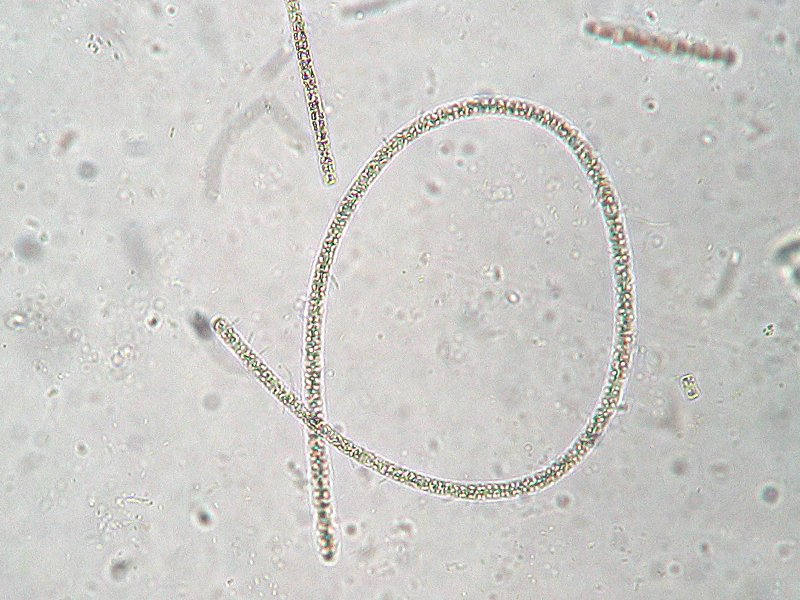
\includegraphics[width=1.7in]{figures/pr.jpeg}\\[-0.5em]
{\tiny (Source: www.limnobotics.ch)}\\
\vfill
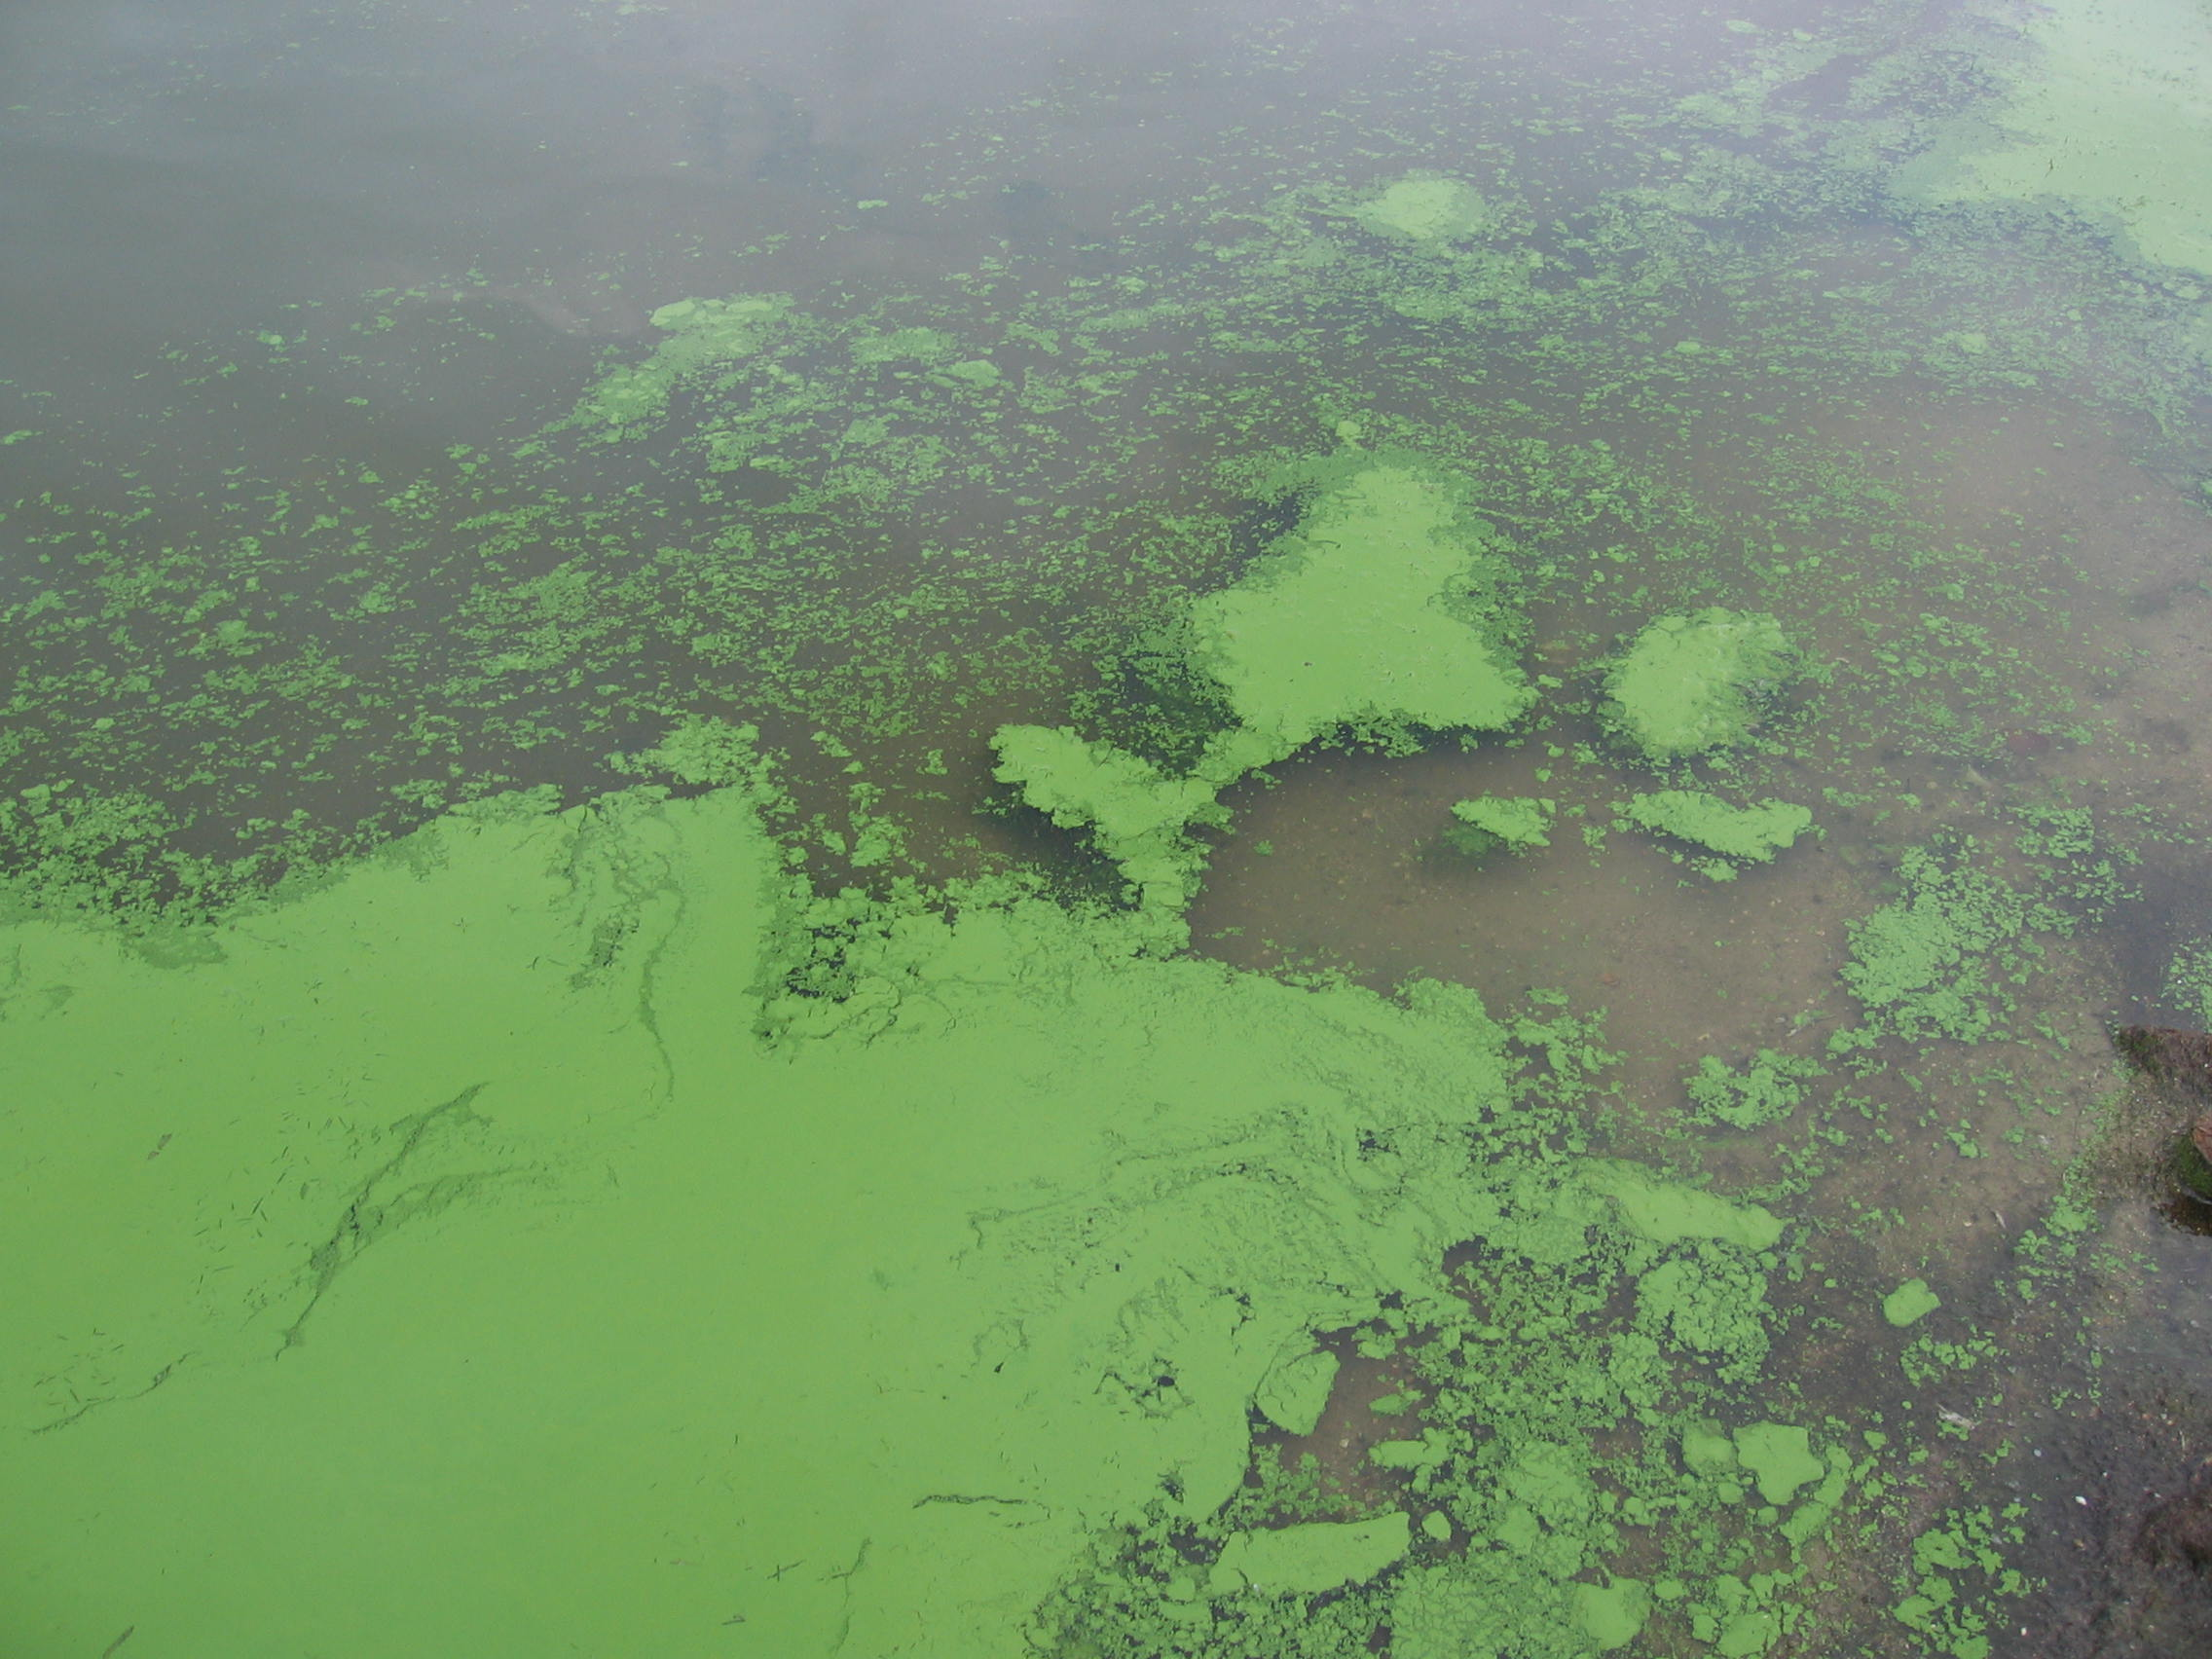
\includegraphics[width=1.7in]{figures/bloom.jpg}\\[-0.5em]
{\tiny (Source: Flickr/Dr. Jennifer L. Graham/U.S. Geological Survey)}
\endminipage

\column{0.6\textwidth}
\minipage[c][0.75\textheight][s]{\columnwidth}
{\small
``The warming waters of one of central Europe's most popular holiday
destinations, Switzerland's Lake Zurich, have created an ideal environment
for a population explosion of algae including \emph{Planktothrix rubescens},
[...]''
\qauth{Scientific American}
\vfill

``\emph{Planktotrhix rubescens} can account for half of the total
phytoplankton biomass in Lake Zurich in summer [...]''
\vfill

``\emph{Planktotrhix rubescens} are among the most important
producers of hepatotoxic microcystins in freshwaters [...]''
\qauth{Silke Van den Wyngaert \emph{et al.}, ASLO, 2011}
\vfill

``Microcystins [...] are cyanotoxins and can be very toxic for plants and
animals including humans.
Their hepatotoxicity may cause serious damage to the liver.''}
\qauth{Wikipedia}
\endminipage
\end{columns}
\end{center}
\end{frame}

\begin{frame}
\begin{center}
\vspace{0.2in}
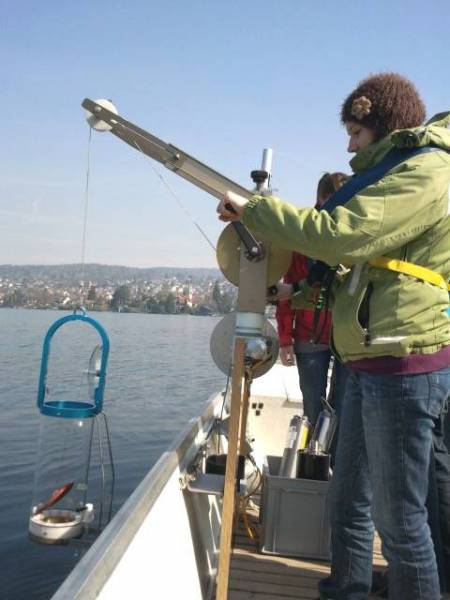
\includegraphics[width=2in]{figures/manual.jpg}\\
{\tiny (Source: www.limnobotics.ch)}
\end{center}
\end{frame}

\begin{frame}
\begin{center}
\vspace{0.2in}
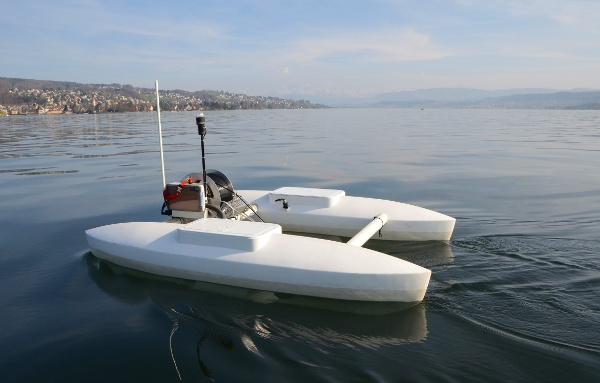
\includegraphics[width=4in]{figures/boat.jpg}\\
{\tiny (Source: www.limnobotics.ch)}
\end{center}
\end{frame}

\begin{frame}
\begin{center}
\vspace{0.2in}
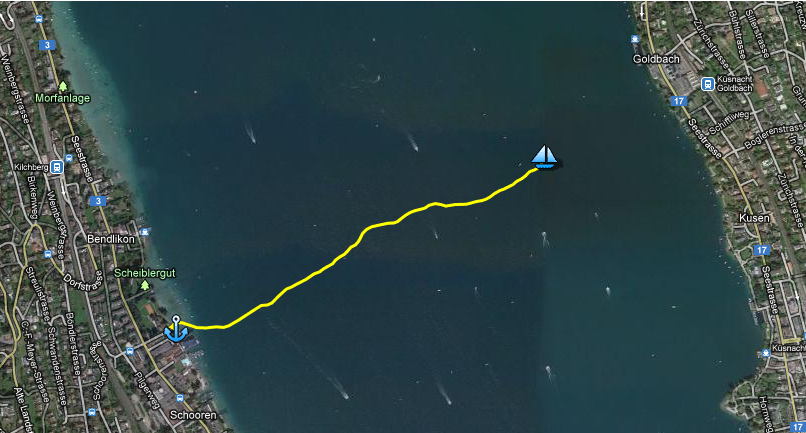
\includegraphics[width=4in]{figures/lake.png}\\
{\tiny (Source: www.limnobotics.ch)}
\end{center}
\end{frame}

\begin{frame}
\begin{center}
\vspace{0.2in}
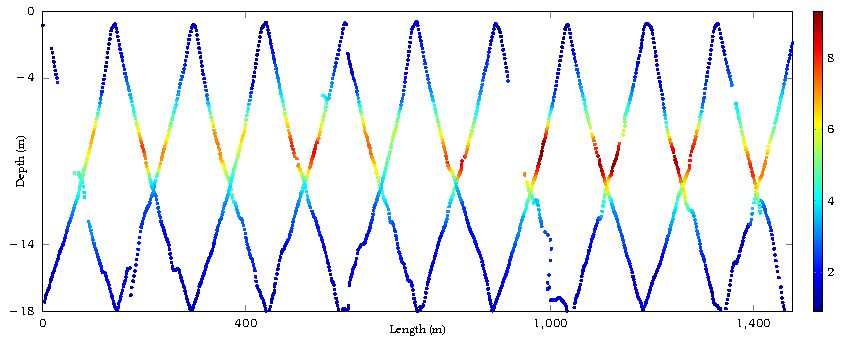
\includegraphics[width=4.7in]{figures/limno_bgape_sc}
\end{center}
\end{frame}

\begin{frame}
\begin{center}
\vspace{0.2in}
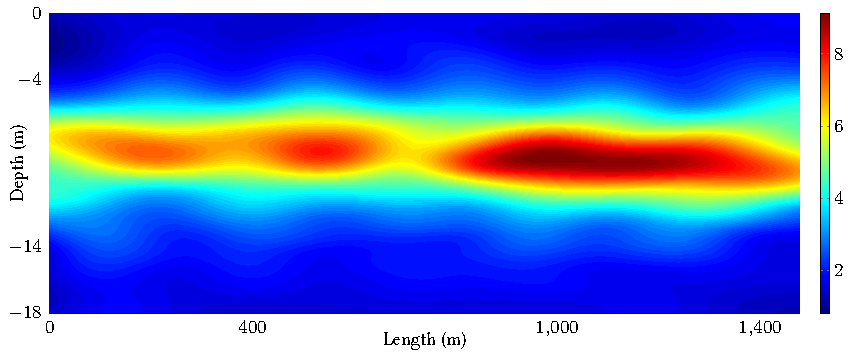
\includegraphics[width=4.7in]{figures/limno_bgape}
\end{center}
\end{frame}

\begin{frame}
\begin{center}
\vspace{0.2in}
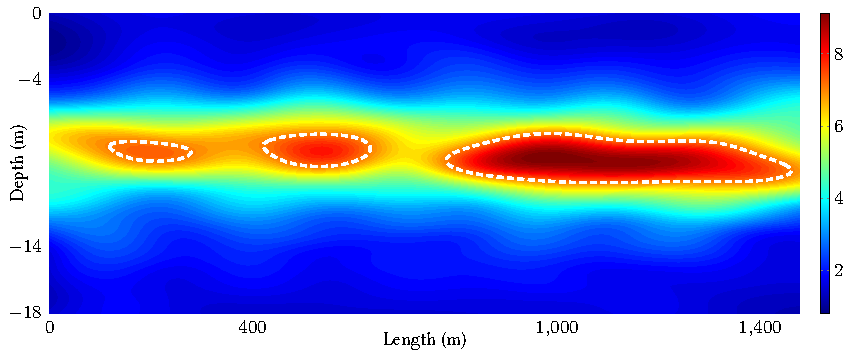
\includegraphics[width=4.7in]{figures/limno_bgape_ls}
\end{center}
\end{frame}

\begin{frame}
\begin{center}
\vspace{0.2in}
\hspace{-2em}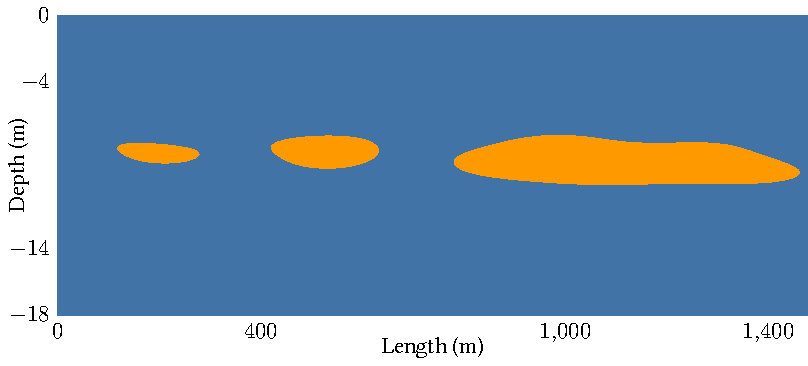
\includegraphics[width=4.45in]{figures/limno_bgape_cl}
\end{center}
\end{frame}

\section{The LSE algorithm}

\begin{frame}
\begin{enumerate}
\item bla
\end{enumerate}
\end{frame}

\section{Extensions}

\begin{frame}
\begin{enumerate}
\item bla
\end{enumerate}
\end{frame}

\section{Results}

\begin{frame}
\begin{enumerate}
\item bla
\end{enumerate}
\end{frame}

\section*{Conclusion}

\begin{frame}
\begin{enumerate}
\item bla
\end{enumerate}
\end{frame}

%\begin{frame}{Make Titles Informative. Use Uppercase Letters.}{Subtitles are optional.}
%  % - A title should summarize the slide in an understandable fashion
%  %   for anyone how does not follow everything on the slide itself.
%
%  \begin{itemize}
%  \item
%    Use \texttt{itemize} a lot.
%  \item
%    Use very short sentences or short phrases.
%  \end{itemize}
%\end{frame}
%
%\begin{frame}{Make Titles Informative.}
%
%  You can create overlays\dots
%  \begin{itemize}
%  \item using the \texttt{pause} command:
%    \begin{itemize}
%    \item
%      First item.
%      \pause
%    \item    
%      Second item.
%    \end{itemize}
%  \item
%    using overlay specifications:
%    \begin{itemize}
%    \item<3->
%      First item.
%    \item<4->
%      Second item.
%    \end{itemize}
%  \item
%    using the general \texttt{uncover} command:
%    \begin{itemize}
%      \uncover<5->{\item
%        First item.}
%      \uncover<6->{\item
%        Second item.}
%    \end{itemize}
%  \end{itemize}
%\end{frame}

%\begin{frame}{Summary}
%
%  % Keep the summary *very short*.
%  \begin{itemize}
%  \item
%    The \alert{first main message} of your talk in one or two lines.
%  \item
%    The \alert{second main message} of your talk in one or two lines.
%  \item
%    Perhaps a \alert{third message}, but not more than that.
%  \end{itemize}
%  
%  % The following outlook is optional.
%  \vskip0pt plus.5fill
%  \begin{itemize}
%  \item
%    Outlook
%    \begin{itemize}
%    \item
%      Something you haven't solved.
%    \item
%      Something else you haven't solved.
%    \end{itemize}
%  \end{itemize}
%\end{frame}


\end{document}


